% \subsubsection{Confusion Matrix}

% A confusion matrix is a compact representation for classification results.
% On the y-axis the truth values $T_*$ of a class are defined and on the x-axis the hypothesis $H_*$ produced by the underlying classifier.
% When the truth class and the hypothesis match, which is the case on the diagonal of the matrix, this results in a \ac{TP}.
% The other case is when the hypothesis does not match the truth value, which can be seen for each class to the left and the right side of the diagonal this is called a \ac{FP}.
% The number of \ac{FN} and \ac{TN} is not presented in the confusion matrix.
% \acp{FN} are the number of missing predictions, which can occur e.g. in object detection when no bounding box is predicted at all.

% \begin{table}
% \begin{center}
% \begin{tabular}{c | c c c c | c}
%     & \textbf{$H_1$} & \textbf{$H_2$} & \textbf{\ldots} & \textbf{$H_C$} & {$\Sigma$} \\
%     \hline
%     $T_1$ & \cellcolor{green}$n_{11}$ & $n_{12}$ & \ldots & $n_{1C}$ & $N_1$\\
%     $T_2$ & $n_{21}$ & \cellcolor{green}$n_{22}$ & \ldots & $n_{2C}$ & $N_2$\\
%     \textbf{$\vdots$} & $\vdots$ & $\vdots$ & \cellcolor{green}$\ddots$ & $\vdots$ & \textbf{$\vdots$} \\
%     $T_C$ & $n_{C1}$ & $n_{C2}$ & \ldots &\cellcolor{green} $n_{CC}$ & $N_C$\\
%     \hline
%     $\Sigma$  & & & & & $N$\\
% \end{tabular}
% \caption{A Confusion Matrix. Truth values are on the y-axis, while the hypothesis (prediction) is on the x-axis. Along the diagonal are the \ac{TP} values.}
% \label{tab:confmat}
% \end{center}
% \end{table}

% In the context of object detection \acp{TP} and \acp{FP} are obtained by measuring the overlap of two bounding boxes, i.e. bounding box $A$ and $B$ are considered to be a \ac{TP} when $IoU(A, B) > threshold$ and the predicted classes of $A$ and $B$ matches, else it is a \ac{FP}.
% After that all assigned \acp{TP} have to be rechecked, such that no ground truth has two matches.
% If such a case occurs the one with the lowest \ac{IoU} with the ground truth bounding box can be reassigned to a \ac{FN}, if again it satisfices the \ac{IoU} criteria.

\subsubsection{True Positive, False Positive, False Negative}
\label{sec:tpfpfn}

To understand the following subsections first the notion of \ac{TP}, \ac{FP} and \ac{FN} should be explained.
A \ac{TP} occurs when the prediction of a network is equal to the underlying ground truth.
Further, a \ac{FP} occurs when the prediction of a network is not equal to the underlying ground truth, normally in terms of that the predicted class differs from the ground truth class, this also includes predictions where a ground truth class is not present at all.
Finally, a \ac{FN} occurs when a prediction is missing completely, so no prediction exists for a ground truth.
In object detection the above definition can't be applied directly.
Since multiple bounding boxes are predicted there has to be a measure of similarity for bounding boxes, to match a ground truth bounding box against a predicted one.
So for example for the \ac{TP} case not only the class of predicted box $A$ and ground truth box $B$ has to match, but also the $IoU(A, B)$ has to be above a certain threshold.

\subsubsection{Precision}

The precision metric (eq. \ref{eq:precision}) states the proportion of all correct identified samples (\ac{TP}) in relation to all positive identified samples.

\begin{equation}
    Precision = \frac{TP}{TP + FP}
    \label{eq:precision}
\end{equation}

\subsubsection{Recall}

The recall metric (eq. \ref{eq:recall}) states the proportion of all correct identified samples in relation to all possible positive samples.

\begin{equation}
    Recall = \frac{TP}{TP + FN}
    \label{eq:recall}
\end{equation}

\subsubsection{F1-Score}

The F1-Score combines precision and recall in one metric as the harmonic mean of both.
It is defined as:

\begin{equation}
    F1 = \frac{2 * recall * precision}{recall + precision}
\end{equation}

\subsubsection{Average Precision (AP)}

\ac{AP} is the most common metric in the context of object detection. It is calculated for each class separately.
It can be calculated by taking a fixed \ac{IoU} threshold and calculating precision and recall with that threshold as it is done in Pascal VOC \cite{map_pascal_voc}, or by taking multiple \ac{IoU} thresholds as it is done in COCO \cite{map_coco}, where the thresholds range from $0.5$ to $0.95$ in $0.05$ steps.
The resulting tuples of (recall, precision) are now sorted ascending by the recall value.
The resulting precision-recall curve could then look like the one in fig. \ref{fig:pr_curve}, this curve is not interpolated.
Normally the precision-recall curve is further interpolated such that it is strictly monotonically decreasing.
The \ac{AP} is then the area under the curve and is calculated
by taking the integral over the domain of the curve (eq. \ref{eq:ap}).

\begin{equation}
    AP = \int_0^1 Precision(Recall) dRecall
    \label{eq:ap}
\end{equation}

\begin{figure}
\begin{center}
    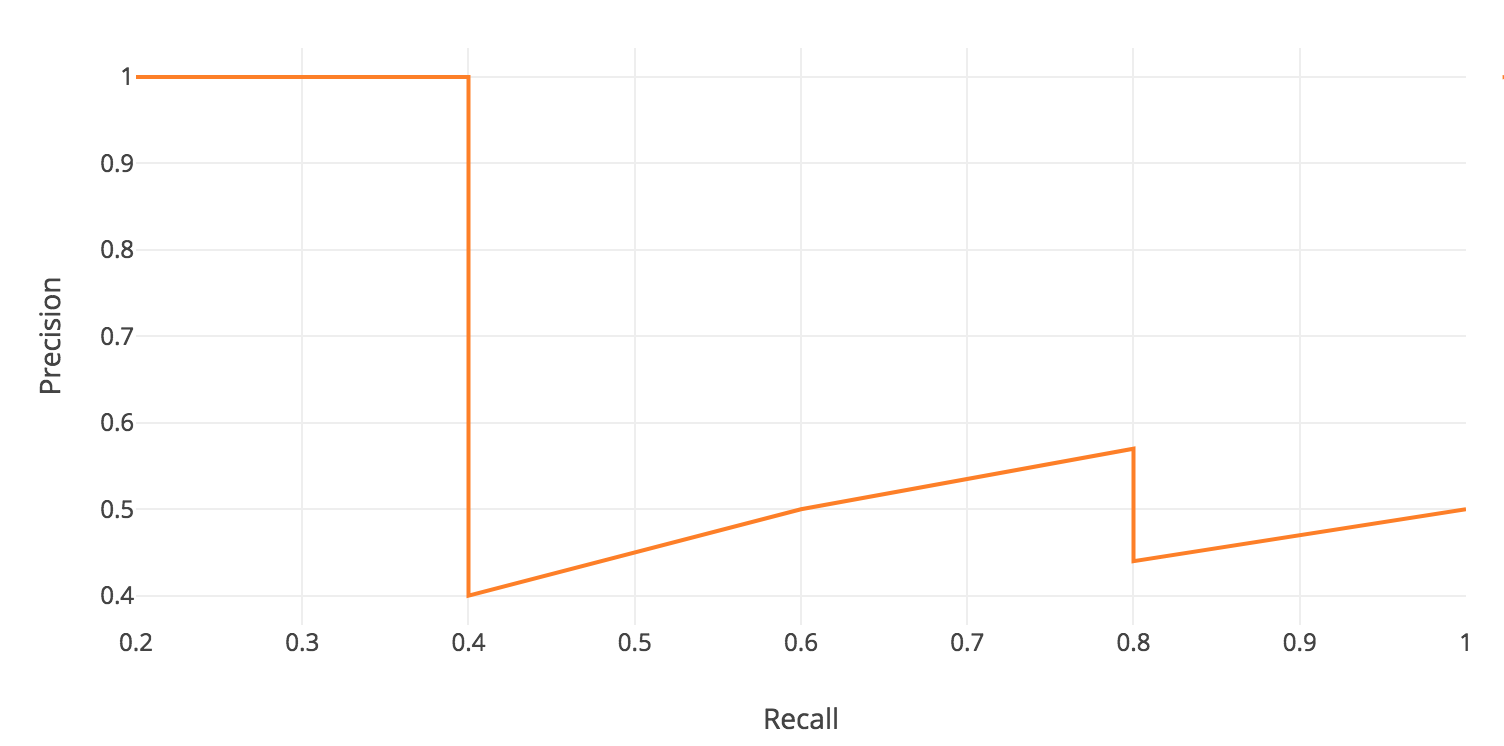
\includegraphics[width=11cm]{imgs/pr_curve.png}
    \caption{Example of a precision-recall curve, where precision and recall were calculated for different \ac{IoU} thresholds and sorted and plotted by their recall values \cite{map_article}. The \ac{AP} is the area under the curve.}
    \label{fig:pr_curve}
\end{center}
\end{figure}

\subsubsection{Mean Average Precision (mAP)}

An extension of the \ac{AP} metric is the \ac{mAP}, which measures overall classification performance for all classes combined.
It is calculated as the mean of all classwise \acp{AP}, where $N$ is the number of classes (eq. \ref{eq:map}).

\begin{equation}
    mAP = \frac{1}{N} \Sigma_{i=1}^N AP_i
    \label{eq:map}
\end{equation}

\subsubsection{Mean Intersection over Union (mIoU)}

\ac{mIoU} is a metric often used in segmentation tasks.
As the name suggests it measures the \ac{IoU} between the predicted mask and the ground truth mask.
Further, the mean of all \ac{IoU} values is calculated over the number of measured samples $N$ and results in the final \ac{mIoU} value (eq. \ref{eq:miou}).

\begin{equation}
    mIoU = \frac{1}{N} \Sigma_{i=0}^{N} IoU_i
    \label{eq:miou}
\end{equation}
